\section{Instruction Sets} 
  
  Let's review what we have so far. From only gates, we have constructed the three main components. 
  \begin{enumerate}
    \item A CPU that can do various arithmetic operations with the ALU and multiplexors. 
    \item A larger memory bank, called RAM, where the CPU can load and store to. 
    \item Since a CPU cannot directly do operations in RAM, a set of registers is built into the CPU and is the only place where the CPU can perform operations.\footnote{which is why it must move data from memory to registers before it can perform operations on it.}
  \end{enumerate}

  While this is physically implemented in hardware, it is probably not the most efficient to take pieces of wires and directly send electrical signals by physically tapping the pins on the processor. What we first need is some \textit{interface} to efficiently communicate with our machine---along with it some sort of standard that both the machine and the human can understand. This naturally introduces an \textit{instruction set}, which is a more human-friendly abstraction above the hardware level. 

  Note that the instruction set is the border between the hardware and software level. Another name for instruction sets is \textit{assembly}, which has many different types of languages depending on the type of CPU. The specific implementations of assembly languages---notably x86, ARM, and RISC-V---will be detailed in my separate assembly notes. This section is to describe the general operations that are considered essential, and we will talk about specific implementations in occasional examples. Note that instructions are simply another layer of abstraction that maps binary sequences to human readable words. 

  \begin{definition}[Instruction Set Architecture]
    The \textbf{instruction set architecture (ISA)} of a CPU is basically a description of what it can do. It specifies the following. 
    \begin{enumerate}
      \item A predetermined set of \textbf{instructions}---also known as \textbf{opcodes}---that describes the operations that the CPU supports. 
      \item The instruction length and decoding, along with its complexity. 
      \item The performance vs power efficiency. 
    \end{enumerate}

    \begin{figure}[H]
      \centering
      \begin{subfigure}[b]{0.48\textwidth}
        \centering
        \begin{lstlisting}
          OPCODE1 arg1 arg2 arg3 
          OPCODE2 arg1 arg2
          ...
          OPCODEn arg1 
        \end{lstlisting}
        \caption{The syntax may differ across ISAs and opcodes, but it is usually the opcode followed by its arguments/operands. The specific opcodes available are usually documented in the ISA's provider page online.}
      \end{subfigure}
      \hfill 
      \begin{subfigure}[b]{0.48\textwidth}
        \centering
        \begin{lstlisting}
          0100 0010 0110 1111 
          0001 000001 010100
          ... 
          1101 1100 00000000 
        \end{lstlisting}
        \caption{Every instruction (opcode and arguments) has a direct binary representation which can entirely fit into a register. In here, we consider a register of 16 bits, and unused bits are zero-padded.}
      \end{subfigure}
      \label{fig:isa_syntax}
    \end{figure}
  \end{definition}

  Note that it only makes sense to talk about the instruction set architecture of some processing unit (e.g. CPU, GPU), and nothing more/less. It does not make sense to talk about the ISA of a computer, and it is usually implied that we are talking about the CPU residing \textit{in} the computer. The ISA is also a subset of the more general \textit{computer architecture}. 

  \begin{example}[CISC vs RISC]
    ISAs can be classified into two types. 
    \begin{enumerate} 
      \item The \textbf{complex instruction set computer} (CISC) is characterized by a large set of complex instructions, which can execute a variety of low-level operations. This approach aims to reduce the number of instructions per program, attempting to achieve higher efficiency by performing more operations with fewer instructions.
      \item The \textbf{reduced instruction set computer} (RISC) emphasizes simplicity and efficiency with a smaller number of instructions that are generally simpler and more uniform in size and format. This approach facilitates faster instruction execution and easier pipelining, with the philosophy that simpler instructions can provide greater performance when optimized.
    \end{enumerate}
  \end{example}

  We should first start off with describing the high level categories of an opcode and an operand. Like higher level programming languages, we can perform operations, do comparisons, and jump to different parts of the code. 

  \begin{definition}[Types of Instructions]
    There are generally three types of instructions. 
    \begin{enumerate} 
      \item \textbf{Data Movement}: These instructions move data between memory and registers or between the registery and registery. Memory to memory transfer cannot be done with a single instruction. 
        \begin{lstlisting} 
          %reg = Mem[address]     # load data from memory into register
          Mem[address] = %reg     # store register data into memory
        \end{lstlisting}
      \item \textbf{Arithmetic Operation}: Perform arithmetic operation on register or memory data. 
        \begin{lstlisting} 
          %reg = %reg + Mem[address]     # add memory data to register
          %reg = %reg - Mem[address]     # subtract memory data from register
          %reg = %reg * Mem[address]     # multiply memory data to register
          %reg = %reg / Mem[address]     # divide memory data from register
        \end{lstlisting}
      \item \textbf{Control Flow}: What instruction to execute next both unconditional and conditional (if statements) ones. With if statements, loops can then be defined. 
        \begin{lstlisting} 
          jmp label     # jump to label
          je label      # jump to label if equal
          jne label     # jump to label if not equal
          jg label      # jump to label if greater
          jl label      # jump to label if less
          call label    # call a function
          ret           # return from a function
        \end{lstlisting}
    \end{enumerate}
  \end{definition}

  \begin{definition}[Types of Operands]

    These are equivalently determined by their \textbf{mode of access}:
    \begin{enumerate} 
      \item \textbf{Immediate addressing} is denoted with a \texttt{\$} sign, e.g. a constant integer data \texttt{\$1}. 
      \item \textbf{Register addressing} is denoted with a \texttt{\%} sign with the following register name, e.g. \texttt{\%rax}.
      \item \textbf{Memory addressing} is denoted with the hexadecimal address in memory, e.g. \texttt{0x034AB}.
    \end{enumerate}
  \end{definition}

\subsection{Data Movement Operations} 

  When we parse an instruction, its operands are one of three things: literals, registers, and memory forms. The method in which we access each type of data is known as a \textbf{mode of access}. These three types are pretty universal, but the syntax in the modes of access vary quite a bit. 

  \begin{definition}[Literals]
    A \textbf{literal} is a constant value, which we will label as \texttt{L} or some other capital letter when specified. 
  \end{definition}

  \begin{definition}[Immediate Addressing]
    A literal is accessed through \textbf{immediate addressing modes}, when the operand of an instruction is a literal \texttt{L}.\footnote{This seems a bit repetitive, saying that \texttt{L} is accessed by \texttt{L}. In our syntax it is, but in other languages, like x86, literals are prepended with \texttt{\$}, e.g. \texttt{\$1} or \texttt{\$0x13}.} 
  \end{definition}

  Every ISA has a predetermined set of registers. 

  \begin{definition}[Registers]
    The set of registers of a $n$-bit ISA correspond to the physical registers on the CPU of bit length $n$. There are two types. 
    \begin{enumerate}
      \item \textit{General-purpose registers}---labeled as \texttt{R1}, \texttt{R2}, ..., \texttt{Ri}---can be used to store any value that the coder wants. 
      \item \textit{Special-purpose registers} are reserved for storing special values and should not in general be used. We will introduce special purpose registers and their notations along the way. 
    \end{enumerate}
  \end{definition}

  One example of a special purpose register is the stack pointer, which always keep track of the next memory location for the CPU to retrieve. We will cover this later, but note that if we were to override the stack pointer (which we have the power to do), then the program will most likely break. Another example is the \textit{frame pointer}, which points to the base of the current stack frame, and \textit{instruction pointers}, which point to the next instruction to be executed. 

  Furthermore, there are general conventions even for general-purpose registers. This is to set some standard that programmers can work with, given that assembly is hard enough to learn on its own.  For example, certain general registers are generally known to store the parameters of a functions. \textit{Return registers} store return values of functions. In order to see which registers are on or off limits, you must refer to the documentation of each language. 

  \begin{example}[Types of Registers]
    Here is a snippet from the \href{https://developer.apple.com/documentation/xcode/writing-arm64-code-for-apple-platforms}{Apple Developer Docs} for ARM64 assembly: The ARM standard delegates certain decisions to platform designers. Apple platforms adhere to the following choices:
    \begin{itemize}
      \item The platforms reserve register x18. Don’t use this register.
      \item The frame pointer register (x29) must always address a valid frame record. Some functions---such as leaf functions or tail calls---may opt not to create an entry in this list. As a result, stack traces are always meaningful, even without debug information.
    \end{itemize}
  \end{example}

  \begin{definition}[Normal/Register Addressing]
    The value residing in a register \texttt{Ri} is accessed through \textbf{normal/register addressing modes}, in the following syntax. 
    \begin{equation}
      \texttt{Reg[Ri]}
    \end{equation}
  \end{definition}

  Finally, we have talked about accessing data on memory banks. By definition, a memory bank must be accessed through its memory address, and fortunately, we have designed our architecture so that all memory addresses can be indexed by a number that fits in our $n$-bit width register. We can refer to this address plus its value at the address as a \textit{memory form}. 

  \begin{definition}[Memory Form]
    A \textbf{memory form} refers to some representation of a memory address. 
  \end{definition}

  Therefore the next addressing mode should be very natural. 

  \begin{definition}[Direct Addressing]
    In \textbf{direct accessing modes}, an instruction contains the memory address to access. We will denote it as 
    \begin{equation}
      \texttt{Mem[L]}
    \end{equation}
  \end{definition}

  Note that the literal \texttt{L} was not interpreted as a value itself, but rather as a memory address. Therefore, if we store \texttt{L} in a register, then we can interpret the contents of a register as sort of like a pointer to some other location in memory. This introduces us the familiar concept in low-level programming languages. There can be multiple levels of indirection here. A register may point to a memory address and a memory bank may itself point to another memory address. 

  \begin{definition}[Pointer]
    A memory device that stores a memory address is said to be a \textbf{pointer}. To access the value at a location in memory, we \textbf{dereference} the pointer as follows. 
    \begin{equation}
      \texttt{Mem[Reg[Ri]]}, \qquad \texttt{Mem[Mem[L]]}
    \end{equation}
    Above, \texttt{Ri} is a pointer since it is a register that contains \texttt{Reg[Ri]}, an address to another memory. Similarly, \texttt{Mem[L]} is a pointer since the value at this location in memory points to another memory address. 
  \end{definition}

  Therefore, there is a duality. A literal \texttt{L} can be interpreted both as a value or a pointer. This allows us to use syntactic sugar to compute offset memories through a technique called \textbf{pointer arithmetic}. The following addressing modes are just fancy names for computing offsetting addresses. 

  \begin{definition}[Offset Addressing]
    Take a base memory address \texttt{B}, an offset \texttt{D}, and a scale factor \texttt{S}.\footnote{We need a scale factor since the word size---the bit length of memory banks---may be several Bytes.} We can access the offset memory address 
    \begin{equation}
      \texttt{Mem[B + S * D]} 
    \end{equation}
    in the following ways.\footnote{The names are very interchangeable depending on context, so rather than just memorizing these, just know that you can always replace literals with addresses, and use them to calculate offsets.}
    \begin{enumerate}
      \item If the base address is a literal and \texttt{D = Reg[Ri]} is stored in a register, i.e. \texttt{Ri} is a pointer, then this is called \textbf{indexed addressing}. 
        \begin{equation}
          \texttt{Mem[B + S * Reg[Ri]]}
        \end{equation}

      \item If the base address \texttt{B = Reg[Rb]} and offset is a literal, then this is called \textbf{displacement addressing}. 
        \begin{equation}
          \texttt{Mem[Reg[Rb] + S * D]}
        \end{equation}

      \item If the base address \texttt{B = Reg[Rb]} and offset is also a pointer \texttt{D = Reg[Ri]}, then this is called \textbf{indirect addressing}. 
      \begin{equation}
        \texttt{Mem[Reg[Rb] + S * Reg[Ri]]}
      \end{equation}
    \end{enumerate}
  \end{definition}

  Note that this is just syntax, and the \texttt{+} and \texttt{*} signs do not mean anything yet. 

  Now that we have developed syntax for accessing data, the next thing to do is to know how to move data around. Let's define a simple operator for this. 

  \begin{definition}[\texttt{mov}]
    The move operation has the following syntax. It is more of a copy rather than a move. 
    \begin{equation}
      \texttt{mov (source) (destination)}
    \end{equation}
    and supports the following combination of operands. 
    \begin{lstlisting}
      mov L       Ri        // move literal L to register Ri
      mov L       Mem[A]    // move literal L to memory address at A
      mov Ri      Rj        // copy value at register Ri to register Rj
      mov Ri      Mem[A]    // move value at register Ri to memory address at A 
      mov Mem[A]  Ri        // move value at memory address A to register Ri 
      mov Mem[A1] Mem[A2]   // move value at memory address A1 to address A2 
    \end{lstlisting}
    Note the following details on the syntax. 
    \begin{enumerate}
      \item We cannot set a literal as the destination, and so there are no operands that support this. 
      \item The syntax for moving the value at register \texttt{Ri} to \texttt{Rj} is not \texttt{mov Reg[Ri] Rj}. 
    \end{enumerate}
  \end{definition}

  Note that when a move instruction is called, the opcode \texttt{mov} along with its operands will get translated into binary. Consider a 16-bit machine with 6-bit opcodes and 5-bit operands. If the opcode for \texttt{mov} is \texttt{111000} and say that we look for the two cases. 
  \begin{enumerate}
    \item We want to move the value at register \texttt{Ri}, which may translate to the binary encoding \texttt{11111}, to the value at register \texttt{Rj}, which may have the binary encoding \texttt{00000}. 
    \item We want to move the literal \texttt{11111} to the value at register \texttt{Rj} with binary encoding \texttt{00000}.  
  \end{enumerate}
  Both scenarios give us the instruction encoding as 
  \begin{equation}
    \texttt{111000 11111 00000}
  \end{equation}
  The CPU---only able to interpret the instruction as a sequence of bits, will not be able to differentiate the two. The solution is to have \textit{different} binary encodings for each version of the \texttt{mov} operation. 

  \begin{example}[\texttt{mov} Opcodes in x86]
    The \texttt{mov} instruction in x86\_64 has the following opcodes. Note that in here, the first operand is the destination 

    \begin{figure}[H]
      \centering 
      \begin{tabular}{|l|l|}
        \hline
        \textbf{Opcode} & \textbf{Description} \\
        \hline
        \texttt{0x88} & mov r/m8, r8 (byte register to memory/register) \\
        \hline
        \texttt{0x89} & mov r/m32/64, r32/64 (32/64-bit register to memory/register) \\
        \hline
        \texttt{0x8A} & mov r8, r/m8 (memory/register to byte register) \\
        \hline
        \texttt{0x8B} & mov r32/64, r/m32/64 (memory/register to 32/64-bit register) \\
        \hline
        \texttt{0xB0-0xB7} & mov r8, imm8 (immediate byte to 8-bit register) \\
        \hline
        \texttt{0xB8-0xBF} & mov r32/64, imm32/64 (immediate to 32/64-bit register) \\
        \hline
        \texttt{0xC6} & mov r/m8, imm8 (immediate byte to memory/register) \\
        \hline
        \texttt{0xC7} & mov r/m32/64, imm32 (immediate to memory/register) \\
        \hline
      \end{tabular}
      \caption{Opcodes for x86.} 
    \end{figure}

    We can see this in the object dump file. 
      
    \begin{figure}[H]
      \centering 
      \begin{lstlisting}
        > objdump -d exit

        exit:     file format elf64-x86-64

        Disassembly of section .text:

        0000000000401000 <_start>:
          401000:	b8 01 00 00 00       	mov    $0x1,%eax
          401005:	bb 12 00 00 00       	mov    $0x12,%ebx
          40100a:	cd 80                	int    $0x80
      \end{lstlisting}
      \caption{} 
    \end{figure}
  \end{example}

  One final note is that in actual implementation, the load (\texttt{ldr}) operation is actually used to move data from memory to registers, while \texttt{mov} is used to move from registers to registers/memory. Memory to memory transfer cannot be done with a single execution. 

\subsection{Arithmetic and Logical Operations}

  Now we start abstracting away the implementations of combinational circuits into a language. 

  \begin{definition}[Flag Register]
    The \texttt{flg} register keep tracks of all this stuff. The most common flags are as follows. 

    \begin{figure}[H]
      \centering 
      \begin{tabular}{|c|l|p{8cm}|}
        \hline
        \textbf{Flag} & \textbf{Name} & \textbf{Description} \\
        \hline
        Z & Zero flag & Indicates that the result of an arithmetic or logical operation (or, sometimes, a load) was zero. \\
        \hline
        C & Carry flag & Enables numbers larger than a single word to be added/subtracted by carrying a binary digit from a less significant word to the least significant bit of a more significant word as needed. It is also used to extend bit shifts and rotates in a similar manner on many processors (sometimes done via a dedicated X flag). \\
        \hline
        S / N & \begin{tabular}[t]{@{}l@{}}Sign flag \\ Negative flag\end{tabular} & Indicates that the result of a mathematical operation is negative. In some processors, the N and S flags are distinct with different meanings and usage: One indicates whether the last result was negative whereas the other indicates whether a subtraction or addition has taken place. \\
        \hline
        V / O / W & Overflow flag & Indicates that the signed result of an operation is too large to fit in the register width using two's complement representation. \\
        \hline
      \end{tabular}
      \caption{Most common CPU status register flags, implemented in almost all modern processors.} 
    \end{figure}

    Some less common flags are shown below. 

    \begin{figure}[H]
      \centering 
      \begin{tabular}{|c|l|p{8cm}|}
        \hline
        \textbf{Flag} & \textbf{Name} & \textbf{Description} \\
        \hline
        H / A / DC & \begin{tabular}[t]{@{}l@{}}Half-carry flag \\ Auxiliary flag \\ Digit carry \\ Decimal adjust flag\end{tabular} & Indicates that a bit carry was produced between the nibbles (typically between the 4-bit halves of a byte operand) as a result of the last arithmetic operation. Such a flag is generally useful for implementing BCD arithmetic operations on binary hardware. \\
        \hline
        P & Parity flag & Indicates whether the number of set bits of the last result is odd or even. \\
        \hline
        I & Interrupt flag & On some processors, this bit indicates whether interrupts are enabled or masked. If the processor has multiple interrupt priority levels, such as the PDP-11, several bits may be used to indicate the priority of the current thread, allowing it to be interrupted only by hardware set to a higher priority. On other architectures, a bit may indicate that an interrupt is currently active, and that the current thread is part of an interrupt handler. \\
        \hline
        S & Supervisor flag & On processors that provide two or more protection rings, one or more bits in the status register indicate the ring of the current thread (how trusted it is, or whether it must use the operating system for requests that could hinder other threads). On a processor with only two rings, a single bit may distinguish Supervisor from User mode. \\
        \hline
      \end{tabular}
      \caption{} 
    \end{figure}
  \end{definition}

  \begin{example}[Flag Registers in x86 and ARM]
    Here are some common flag register implementations.
    \begin{enumerate}
      \item In x86, the \texttt{FLAGS} register contains. 
      \item In ARM, the \texttt{NZCV} register stores the sign, zero, carry, and overflow flags. 
      \item In RISC-V, comparison instructions store the comparison result in a general-purpose register, and conditional branches act based on the value in the general purpose register. 
      \item In MIPS, we do not use a dedicated flag register. 
    \end{enumerate}
  \end{example}
  
  With the flag registers, we can have a complete implementation of the following. 

  \begin{definition}[Addition]
    The addition operation performs arithmetic addition and stores the result in the destination.
    \begin{equation}
      \texttt{add (source) (destination)}
    \end{equation}
    and supports the following combination of operands.
    \begin{lstlisting}
      add L       Ri        // add literal L to register Ri
      add L       Mem[A]    // add literal L to value at memory address A
      add Ri      Rj        // add value at register Ri to register Rj
      add Ri      Mem[A]    // add value at register Ri to value at memory address A
      add Mem[A]  Ri        // add value at memory address A to register Ri
      add Mem[A1] Mem[A2]   // add value at memory address A1 to value at address A2
    \end{lstlisting}
    Note the following details on the syntax.
    \begin{enumerate}
      \item The destination operand is modified to contain the sum of source and destination.
      \item We cannot set a literal as the destination, and so there are no operands that support this.
      \item The operation affects processor flags including zero, carry, overflow, and sign flags.
    \end{enumerate}
  \end{definition}

  \begin{definition}[Addition with Carry]
    
  \end{definition}

  \begin{definition}[Subtraction]
    The subtraction operation performs arithmetic subtraction and stores the result in the destination.
    \begin{equation}
      \texttt{sub (source) (destination)}
    \end{equation}
    and supports the following combination of operands.
    \begin{lstlisting}
      sub L       Ri        // subtract literal L from register Ri
      sub L       Mem[A]    // subtract literal L from value at memory address A
      sub Ri      Rj        // subtract value at register Ri from register Rj
      sub Ri      Mem[A]    // subtract value at register Ri from value at memory address A
      sub Mem[A]  Ri        // subtract value at memory address A from register Ri
      sub Mem[A1] Mem[A2]   // subtract value at memory address A1 from value at address A2
    \end{lstlisting}
    Note the following details on the syntax.
    \begin{enumerate}
      \item The destination operand is modified to contain the difference (destination - source).
      \item We cannot set a literal as the destination, and so there are no operands that support this.
      \item The operation affects processor flags including zero, carry, overflow, and sign flags.
    \end{enumerate}
  \end{definition}

  \begin{definition}[Multiplication]
    The multiplication operation performs arithmetic multiplication and stores the result in the destination.
    \begin{equation}
      \texttt{mul (source) (destination)}
    \end{equation}
    and supports the following combination of operands.
    \begin{lstlisting}
      mul L       Ri        // multiply register Ri by literal L
      mul L       Mem[A]    // multiply value at memory address A by literal L
      mul Ri      Rj        // multiply register Rj by value at register Ri
      mul Ri      Mem[A]    // multiply value at memory address A by value at register Ri
      mul Mem[A]  Ri        // multiply register Ri by value at memory address A
      mul Mem[A1] Mem[A2]   // multiply value at address A2 by value at address A1
    \end{lstlisting}
    Note the following details on the syntax.
    \begin{enumerate}
      \item The destination operand is modified to contain the product of source and destination.
      \item We cannot set a literal as the destination, and so there are no operands that support this.
      \item The operation may produce results larger than register width, affecting overflow flags.
    \end{enumerate}
  \end{definition}

  \begin{definition}[Division]
    The division operation performs arithmetic division and stores the result in the destination.
    \begin{equation}
      \texttt{div (source) (destination)}
    \end{equation}
    and supports the following combination of operands.
    \begin{lstlisting}
      div L       Ri        // divide register Ri by literal L
      div L       Mem[A]    // divide value at memory address A by literal L
      div Ri      Rj        // divide register Rj by value at register Ri
      div Ri      Mem[A]    // divide value at memory address A by value at register Ri
      div Mem[A]  Ri        // divide register Ri by value at memory address A
      div Mem[A1] Mem[A2]   // divide value at address A2 by value at address A1
    \end{lstlisting}
    Note the following details on the syntax.
    \begin{enumerate}
      \item The destination operand is modified to contain the quotient (destination ÷ source).
      \item We cannot set a literal as the destination, and so there are no operands that support this.
      \item Division by zero typically triggers an exception or sets error flags.
    \end{enumerate}
  \end{definition}

  \begin{definition}[Increment, Decrement]
    The increment and decrement operations add or subtract 1 from the operand.
    \begin{align*}
      & \texttt{inc (operand)} 
      & \texttt{dec (operand)}
    \end{align*}
    and support the following operands.
    \begin{lstlisting}
      inc Ri        // increment register Ri by 1
      inc Mem[A]    // increment value at memory address A by 1
      dec Ri        // decrement register Ri by 1
      dec Mem[A]    // decrement value at memory address A by 1
    \end{lstlisting}
    Note the following details on the syntax.
    \begin{enumerate}
      \item These are unary operations that modify the operand in place.
      \item Literals cannot be used as operands since they cannot be modified.
      \item The operations affect flags but typically preserve the carry flag.
    \end{enumerate}
  \end{definition}

  \begin{definition}[Negation]
    The negation operation performs two's complement negation of the operand.
    \begin{equation}
      \texttt{neg (operand)}
    \end{equation}
    and supports the following operands.
    \begin{lstlisting}
      neg Ri        // negate value in register Ri
      neg Mem[A]    // negate value at memory address A
    \end{lstlisting}
    Note the following details on the syntax.
    \begin{enumerate}
      \item This is a unary operation that modifies the operand in place.
      \item Literals cannot be used as operands since they cannot be modified.
      \item The operation sets flags based on the result, including overflow for minimum values.
    \end{enumerate}
  \end{definition}

  \begin{definition}[Bitwise Operations]
    The bitwise operations perform logical operations on operands bit by bit.
    \begin{align*}
      & \texttt{and (source) (destination)} \\ 
      & \texttt{or (source) (destination)} \\
      & \texttt{xor (source) (destination)}
    \end{align*}
    and support the following combination of operands.
    \begin{lstlisting}
      and L       Ri        // bitwise AND register Ri with literal L
      or  L       Mem[A]    // bitwise OR value at memory address A with literal L
      xor Ri      Rj        // bitwise XOR register Rj with value at register Ri
      and Ri      Mem[A]    // bitwise AND value at memory address A with register Ri
      or  Mem[A]  Ri        // bitwise OR register Ri with value at memory address A
      xor Mem[A1] Mem[A2]   // bitwise XOR value at address A2 with value at address A1
    \end{lstlisting}
    Note the following details on the syntax.
    \begin{enumerate}
      \item The destination operand is modified to contain the result of the logical operation.
      \item We cannot set a literal as the destination, and so there are no operands that support this.
      \item These operations clear the carry and overflow flags, setting zero and sign flags.
    \end{enumerate}
  \end{definition}

  \begin{definition}[Bitshift]
    The bitshift operations shift bits left or right by a specified number of positions.
    \begin{equation}
      \texttt{shl (count) (operand)} \quad \texttt{shr (count) (operand)}
    \end{equation}
    and support the following combination of operands.
    \begin{lstlisting}
      shl L       Ri        // shift register Ri left by L positions
      shr L       Mem[A]    // shift value at memory address A right by L positions
      shl Ri      Rj        // shift register Rj left by value in register Ri
      shr Ri      Mem[A]    // shift value at memory address A right by value in register Ri
    \end{lstlisting}
    Note the following details on the syntax.
    \begin{enumerate}
      \item The operand is modified to contain the shifted result.
      \item Left shift (shl) multiplies by powers of 2; right shift (shr) divides by powers of 2.
      \item The carry flag receives the last bit shifted out of the operand.
    \end{enumerate}
  \end{definition}

  \begin{definition}[Unconditional Jumps]
    The unconditional jump operation transfers control to a specified address.
    \begin{equation}
      \texttt{jmp (target)}
    \end{equation}
    and supports the following target specifications.
    \begin{lstlisting}
      jmp L         // jump to literal address L
      jmp Ri        // jump to address stored in register Ri
      jmp Mem[A]    // jump to address stored at memory address A
      jmp Label     // jump to labeled instruction
    \end{lstlisting}
    Note the following details on the syntax.
    \begin{enumerate}
      \item This operation unconditionally transfers control, updating the program counter.
      \item Labels are resolved to addresses during assembly or linking.
      \item No processor flags are affected by the jump operation itself.
    \end{enumerate}
  \end{definition}

  \begin{definition}[Compare]
    The compare operation performs subtraction but only sets flags without modifying operands.
    \begin{equation}
      \texttt{cmp (source) (destination)}
    \end{equation}
    and supports the following combination of operands.
    \begin{lstlisting}
      cmp L       Ri        // compare register Ri with literal L
      cmp L       Mem[A]    // compare value at memory address A with literal L
      cmp Ri      Rj        // compare register Rj with value at register Ri
      cmp Ri      Mem[A]    // compare value at memory address A with value at register Ri
      cmp Mem[A]  Ri        // compare register Ri with value at memory address A
      cmp Mem[A1] Mem[A2]   // compare value at address A2 with value at address A1
    \end{lstlisting}
    Note the following details on the syntax.
    \begin{enumerate}
      \item Neither operand is modified; only processor flags are set based on (destination - source).
      \item We cannot set a literal as the destination, and so there are no operands that support this.
      \item Sets zero, carry, overflow, and sign flags for use by conditional jump instructions.
    \end{enumerate}
  \end{definition}

  \begin{definition}[Conditional Jump]
    The conditional jump operation transfers control to a specified address based on processor flags.
    \begin{equation}
      \texttt{jcc (target)}
    \end{equation}
    where \texttt{cc} represents condition codes, and supports the following target specifications.
    \begin{lstlisting}
      je  L         // jump if equal (zero flag set)
      jne L         // jump if not equal (zero flag clear)
      jl  L         // jump if less than (sign != overflow)
      jg  L         // jump if greater than (zero clear and sign == overflow)
      jc  L         // jump if carry set
      jo  L         // jump if overflow set
      js  L         // jump if sign set
    \end{lstlisting}
    Note the following details on the syntax.
    \begin{enumerate}
      \item Control transfers only if the specified condition is met; otherwise execution continues.
      \item Conditions are based on flags set by previous operations like compare or arithmetic.
      \item Common conditions include equality, inequality, and signed/unsigned comparisons.
    \end{enumerate}
  \end{definition}

\subsection{Code and Data Segments}

  Okay, now that we are familiar with the syntax, let's step back to consider how a series of bits are actually converted into code. Given a program, it must work with data, either to store its own code or to access data from memory itself. Whenever there is data, there exists memory, and whenever there is memory, there is the \textit{address} where it is located in. 

  \begin{definition}[Address Space]
    An \textbf{address space} is the range of memory addresses available to a program or a process. Each address space of a program is also called a \textit{segment}. 
  \end{definition}

  The program itself---i.e. the list of instructions---is also data, and so it will be stored in some address space. We have a name for this. 

  \begin{definition}[Text/Code Segment]
    The \textbf{text/code segment} is the address space where the program instructions are stored. It is readable, executable, and of fixed size. It is not writable. 
  \end{definition}

  Okay, so assume that we have the binary encodings of instructions in the text segment, along with the relevant data in the data segment. The CPU is apparently supposed to execute each line of instruction, but 

  \begin{definition}[Instruction Pointer]
    The \textbf{instruction pointer}, which we will denote \texttt{ip}, is a register that stores the address of the next instruction to execute. 
  \end{definition}

  \begin{example}[Execution of Simple Program]

  \end{example}

  \begin{definition}[Data Segment]
    The \textbf{data segment} is the address space where static global variables are stored. It is readable and writable, but not executable.
  \end{definition}

  \begin{definition}[Read Only Data Segment]
    The \textbf{read only data segment}, also known as \textbf{rodata}, is the address space that stores read-only data, i.e. constants. 
  \end{definition}

  These two address spaces are so important that every script written in assembly must specify this. Having no data segment implies that the data segment is empty. 

  \begin{figure}[H]
    \centering
    \begin{subfigure}[b]{0.48\textwidth}
      \centering
      \begin{lstlisting}
        .section .text
        .globl _start

        _start:
          movl $1, %eax 
          movl $0, %ebx 
          int $0x80  
      \end{lstlisting}
      \caption{x86 assembly}
    \end{subfigure}
    \hfill 
    \begin{subfigure}[b]{0.48\textwidth}
      \centering
      \begin{lstlisting}
      \end{lstlisting}
      \caption{ARMv8 assembly}
    \end{subfigure}
    \caption{Every script must have a text section.}
  \end{figure}

  At this point, we introduced the text and data segments as simply some blocks of memory that are allocated before a program starts executing. We will see the full significance of this segments soon. 

\subsection{Stack Memory} 

  Say you are working with an architecture consisting of 32 8-bit registers. You might be working on a program that---during runtime---works with a lot more than just 32 numbers. To solve this, you take advantage of the large pool of RAM that you have already built for yourself. Say you want to store \texttt{0x18} originally in register \texttt{r1} into memory. If you do it, then you will have to store the address of \texttt{0x18} \textit{somewhere} in one of your registers. Therefore you have simply replaced the value with its address and have not saved any space at all! In fact, it is counterproductive since now you have to wait for slow access times into the memory. \footnote{If you read up on the implementation of arrays in my DSA notes, you might think of putting them into a list, storing the front of the array in memory, and having a special terminating character indicating the end of an array. But not all data structures can---nor should---be nicely formatted in this list.}

  Designing the memory so that it works like a \hyperref[dsa-def:stack]{stack} data structure turns out to solve this problem, along with other ones such as function call traces. In fact, the stack is so important that is pretty much universal across all computer architectures. The general idea is to simulate intermediate storage by pushing and popping temporary variables onto the stack. The stack pointer is \textit{not} a fundamental part of memory since memory is just an array of Bytes. It is a part of the ISA. 

  \begin{definition}[Stack Memory/Segment]
    The \textbf{stack memory} is an address space that stores 
    \begin{enumerate}
      \item \textit{Intermediate calculations} 
      \item \textit{Return addresses}
      \item \textit{Local }
    \end{enumerate}
  \end{definition}

  The main API of the stack is at the top address, which is at the \textit{stack pointer}. 

  \begin{definition}[Stack Pointer]
    The \textbf{stack pointer} is a register---denoted \texttt{sp}---that stores the address of the top of the stack. 
  \end{definition}

  \begin{definition}[Push, Pop]
    The push and pop operations manage data on the stack using the stack pointer.
    \begin{equation}
      \texttt{push (operand)} \quad \texttt{pop (operand)}
    \end{equation}
    and support the following operands.
    \begin{lstlisting}
      push L        // push literal L onto stack
      push Ri       // push value in register Ri onto stack
      push Mem[A]   // push value at memory address A onto stack
      pop Ri        // pop top of stack into register Ri
      pop Mem[A]    // pop top of stack into memory address A
    \end{lstlisting}
    Note the following details on the syntax.
    \begin{enumerate}
      \item Push decrements the stack pointer then stores the value; pop retrieves then increments.
      \item We cannot pop into a literal since literals cannot be modified.
      \item Stack grows downward in memory (higher addresses to lower addresses).
    \end{enumerate}
  \end{definition}

  \begin{definition}[Base Pointer]
    
  \end{definition}

  \begin{definition}[Call, Return]
    The call and return operations manage function invocation and return.
    \begin{equation}
      \texttt{call (target)} \quad \texttt{ret}
    \end{equation}
    and support the following target specifications for call.
    \begin{lstlisting}
      call L         // call function at literal address L
      call Ri        // call function at address stored in register Ri
      call Mem[A]    // call function at address stored at memory address A
      call Label     // call labeled function
      ret            // return from current function
    \end{lstlisting}
    Note the following details on the syntax.
    \begin{enumerate}
      \item Call pushes the return address onto the stack then jumps to the target.
      \item Return pops the return address from the stack and jumps to it.
      \item The stack pointer must be properly maintained for correct return behavior.
    \end{enumerate}
  \end{definition}

\subsection{Functions and Control Transfer}

  These are really the three basic functions needed to do anything in assembly, but let's talk about an important implementation called the \textbf{control transfer}. Say that you want to compute a function. 
  \begin{enumerate}
    \item Then we must retrieve the data from the memory. 
    \item We must load it into our registers in the CPU and perform some computation. 
    \item Then we must store the data back into memory. 
  \end{enumerate}

  Let’s begin with a refresher on how the call stack is managed. Recall that \texttt{\%rsp} is the stack pointer and always points to the top of the stack. The register \texttt{\%rbp} represents the base pointer (also known as the frame pointer) and points to the base of the current stack frame. The stack frame (also known as the activation frame or the activation record) refers to the portion of the stack allocated to a single function call. The currently executing function is always at the top of the stack, and its stack frame is referred to as the active frame. The active frame is bounded by the stack pointer (at the top of stack) and the frame pointer (at the bottom of the frame). The activation record typically holds local variables for a function.

  \begin{figure}[H]
    \centering 
    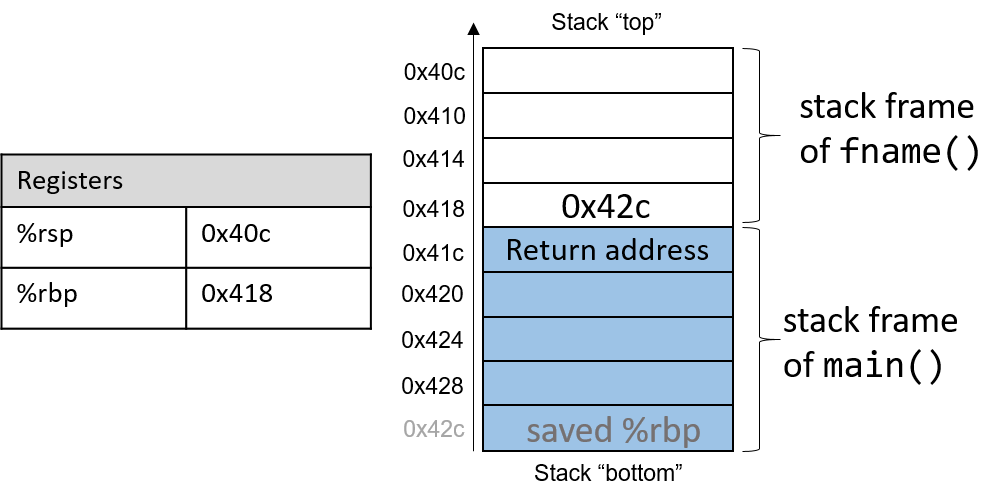
\includegraphics[scale=0.6]{img/stackFrame.png}
    \caption{The current active frame belongs to the callee function (fname). The memory between the stack pointer and the frame pointer is used for local variables. The stack pointer moves as local values are pushed and popped from the stack. In contrast, the frame pointer remains relatively constant, pointing to the beginning (the bottom) of the current stack frame. As a result, compilers like GCC commonly reference values on the stack relative to the frame pointer. In Figure 1, the active frame is bounded below by the base pointer of fname, which is stack address 0x418. The value stored at address 0x418 is the "saved" \texttt{\%rbp} value (0x42c), which itself is an address that indicates the bottom of the activation frame for the main function. The top of the activation frame of main is bounded by the return address, which indicates where in the main function program execution resumes once the callee function fname finishes executing. }
    \label{fig:stack_frame_management}
  \end{figure}


  Once we have done this we are really done. Formally, this is called Turing complete (?). 

  \begin{definition}[Control Transfers]
    We list some. 
    \begin{enumerate}
      \item Push 
      \item Pop 
      \item Call to call a function 
      \item Return to return from a function 
      \item Continue 
      \item Get out of stack with leave.  
    \end{enumerate}
  \end{definition}

  \begin{example}[Control Transfer Example]
    We show this with a minimal example with psuedocode. 
  \end{example}


  \begin{example}[Multiple Functions Example]
    Now what happens if there are multiple functions calling each other? Take a look at the following example with two functions. 
    
  \end{example}

  There is a bit of a concern here from the previous example. The main function had two functions that returned two values. As the subfunction stack frame is removed from the stack, the return value is stored in the \texttt{\%rax} register. If another function is called right after, then the return value of the second function will overwrite that of the previous one. This was not a problem in the previous example since the return value of the \texttt{assign} function was not used. However, if it was, then the return value of the \texttt{adder} function would have overwritten it. This is known as register saving. 
  \begin{enumerate}
    \item For \textbf{caller-saved registers}, the caller function is responsible for saving the value of the register before calling a function and restoring it after the function returns. The caller should save values in its stack frame before calling the callee function, e.g. by pushing all the return values of each callee in the caller stack frame. Then it will restore values after the call. 

    \begin{center}
      \textit{Therefore, if we have a set of registers $\{\texttt{\%reg}\}$, the caller must take everything and push them in the caller stack frame. Then it will restore them after the call.}
    \end{center}

    \item For \textbf{callee-saved registers}, it is the callee's responsibility to save any data in these registers before using the registers. 

      \begin{center} 
        \textit{Therefore, if we have a set of registers $\{\texttt{\%reg}\}$, then inside the callee stack frame, the callee must take everything and push them in the callee stack frame. Once it computes the final return value, then it will restore all the saved register values from the callee stack frame back into the registers for the caller to use.}
      \end{center}
  \end{enumerate}

  Ideally, we want \textit{one} calling convention to simply separate implementation details between caller and callee. In general, however, neither is best. If the caller isn't using a register, then caller-save is better, and if callee doesn't need a register, then callee-save is better. If we do need to save, then callee save generally makes smaller programs, so we compromise and use a combination of both caller-save and callee-save. 

\subsection{Heap Memory}

\subsection{Assembling and Linking}

  The conversion of assembly code into a full binary executable is done through a two step process. First, the code is \textit{assembled} into a set of \textit{object files}, and then these object files are \textit{linked} into a binary executable.\footnote{Common assemblers are \texttt{gas}, \texttt{as} and common linkers are \texttt{ld} (GNU linker) or \texttt{lld} (LLVM linker).}

